\section{Study Area}

\begin{figure}[!t]
  \vspace{-0.5cm}
  \centering
  \subfigure[Map of Portugal and the study area highlighted with the
  red rectangle.]{\label{fig:po-map}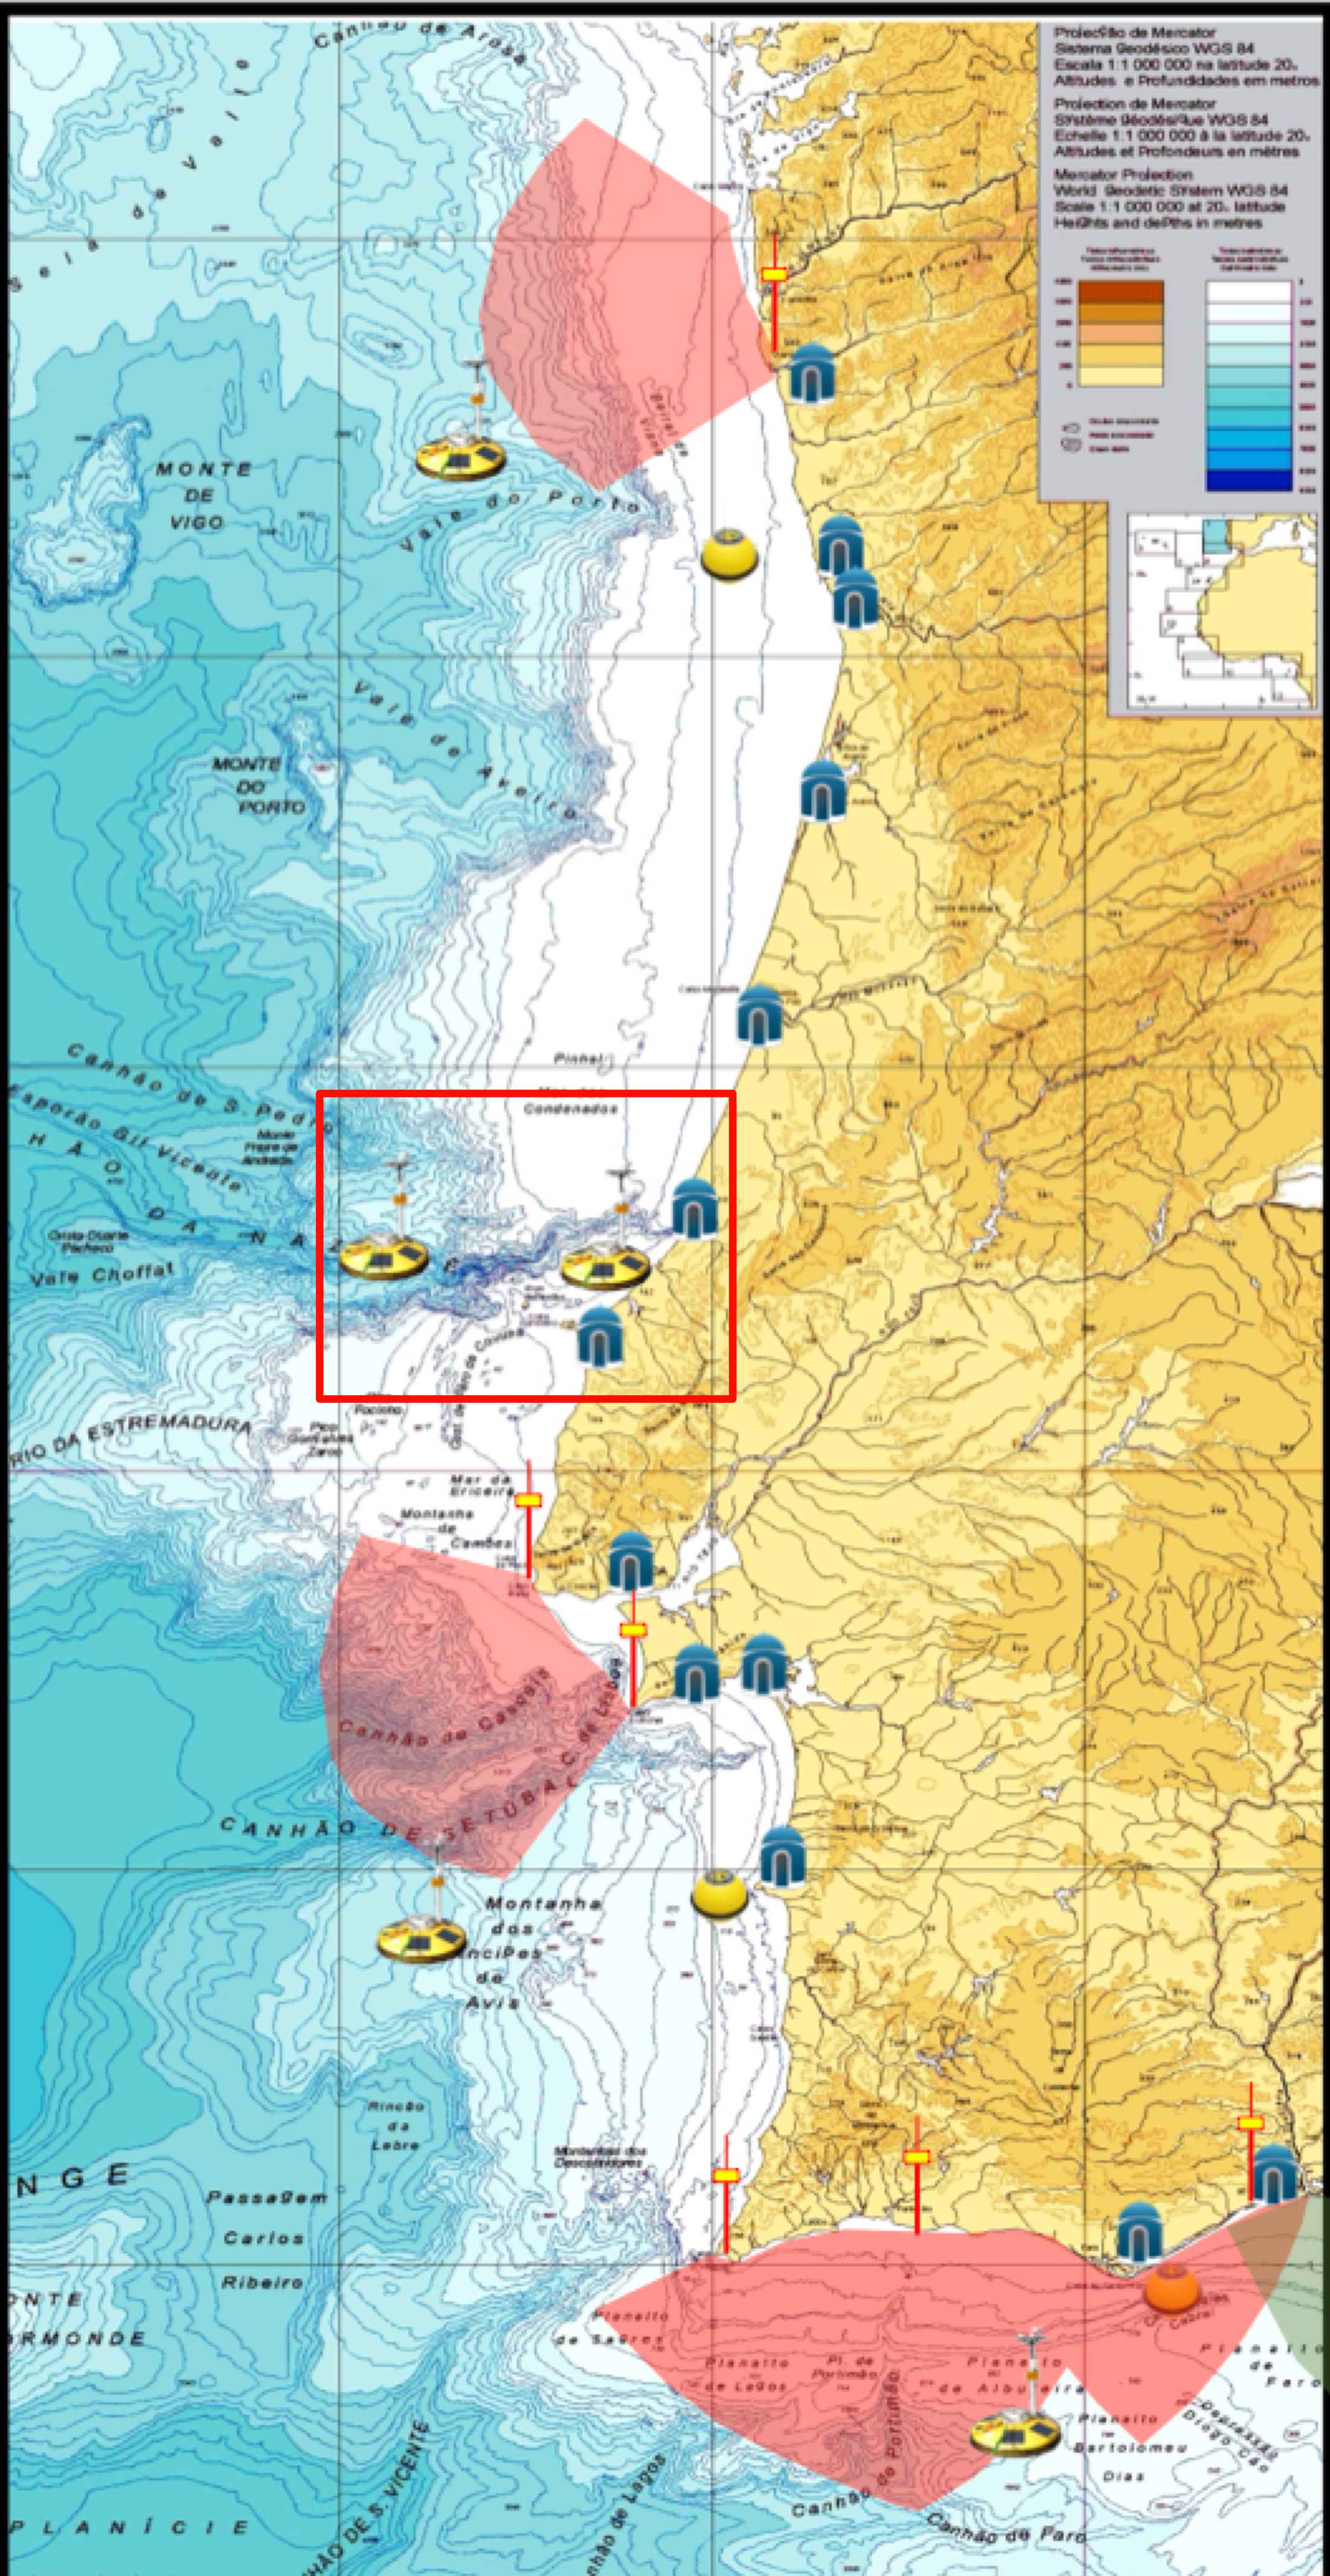
\includegraphics[scale=0.5]{fig/po-map.jpeg}}
  \hspace{+0.3cm}
  \subfigure[Zoomed in bathymetry showing the \naz canyon-Berlengas
  area (isobaths with depth in meters) and its environment including
  the placement of
  buoys.]{\label{fig:domain}\includegraphics[scale=0.55]{fig/domain.jpg}}
  \caption{\subref{fig:po-map} \& \subref{fig:domain} show detailed
    views of the study area for \proj off the coast of mainland
    Portugal. The \naz Canyon is a significant feature of this area
    and a driver for the bio-geophysics of the domain.}
  \label{fig:studyarea-1}
\end{figure}

The study was conducted in the coastal ocean off central Portugal,
focusing on the region influenced by the \naz Canyon (39.2$^{\circ}$
-39.9$^{\circ}$N) (Fig. \ref{fig:studyarea-1}). This area is shaped by
strong topographic contrasts, including the transition from the wide
Estremadura Plateau to the narrower shelf to the north, the long and
narrow \naz submarine canyon that incises the shelf and extends more
than 200 km offshore, and the Berlengas archipelago, a UNESCO
Biosphere Reserve with high ecological value. These features
contribute to enhanced biological productivity and biodiversity, and
strongly modulate physical and biogeochemical processes in the region.

Freshwater inputs from major rivers, such as the Tagus, have only a
limited direct impact on the area. In contrast, smaller rivers and the
\'{O}bidos lagoon can episodically deliver low-salinity, nutrient-rich
plumes to the shelf. Circulation is controlled by seasonal wind forcing
associated with the Azores High, with persistent upwelling-favorable
northerly winds in summer and frequent downwelling episodes in winter
under southerly winds. The interplay between canyon topography, shelf
circulation, and atmospheric forcing generates complex mesoscale
dynamics, intensified tidal currents, and internal wave activity that
promote strong vertical mixing and cross-shelf exchanges
\cite{martins10,quaresma07}.

The combination of sharp bathymetric gradients, variable forcing, and
rich physical–biogeochemical interactions makes the \naz Canyon region
an ideal natural laboratory to test adaptive observation strategies. In
particular, its dynamic environment poses both opportunities and
challenges for the \proj experiment, providing a representative coastal
setting in which to evaluate how model-based uncertainty projections can
guide adaptive sampling and assimilation to improve ocean model
predictive skill.
